JotForm is an international company, having offices in San Francisco, Izmir, and Ankara. Managerial
staff is primarily located in Ankara office, which is also the home for the main R\&D hub for the company. \\
\begin{figure}[hbt!]
    \centering
    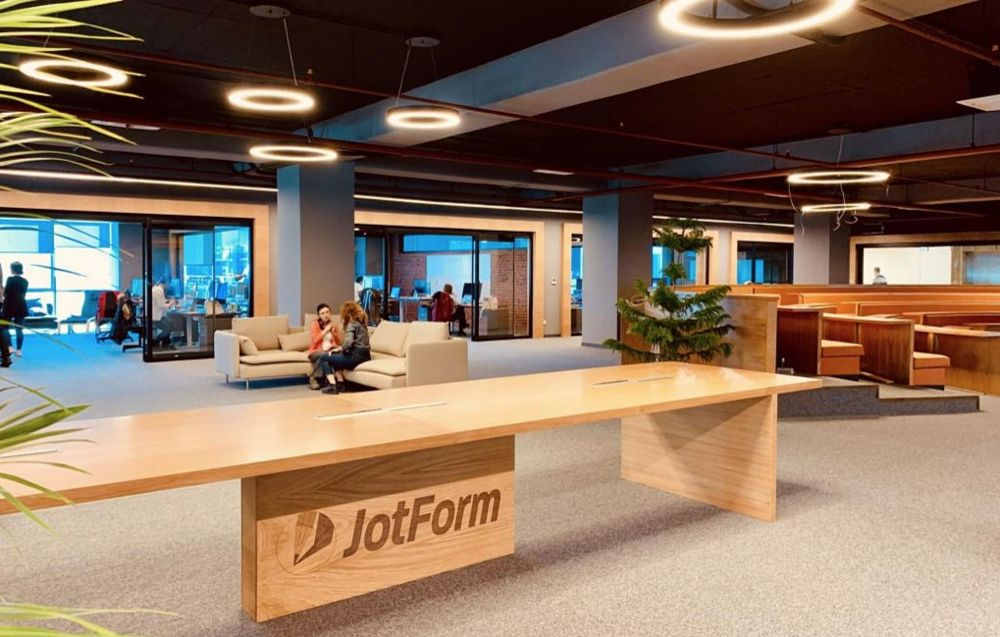
\includegraphics[width=0.9\textwidth]{Images/new-turkey-office.jpg}
    \caption{A View From JotForm's Ankara Offices}
    \label{fig:JFMAnkara}
\end{figure} \\
\subsection{Structure of the company}
In JotForm, employees are operating in teams, named by themselves, such as Amplify, Hermes and so on. The main responsibility of a team is not divided between different products of the company. This way, they can keep their focus, and work more reliably as a team. A team, for example, may work on Form Builder for a certain amount of time, and not in other products such as PDF Editor. This allows for an efficitent \textbf{Agile} work environment. \\
On fridays, all teams from Izmir and Ankara offices of JotForm come together for a meet, called the Demo Day. This facilitates for the presentations of the work done in the week for each team. This day is also the day for us interns to perform their presentations about their projects.

\subsection{Products offered by JotForm}
\subsubsection{Form Builder}
Form Builder tool is the main product of the company. Offering a drag-and-drop interface for creating forms,
analyzing data easily and making the analysis of the results from the form easier (using JotForm Sheets) is the main focus of the company. Since 2006, the founding of the company, they operate a Form Builder interface, which is active to this day. Main differences from competitors such as Google Sheets is the ease of use, and options for payment such as PayPal, Stripe etc. , which makes the product a standalone candidate for e-commerce websites, handling payments and billing information all by itself.

\subsubsection{PDF Editor}
In the last year, JotForm offices in Ankara started a project on PDF documents. Since the main focus of the company is on the forms, and customers repeatedly reporting that they need to convert their PDF forms to some online form, a team in Ankara office has built a tool for the purpose. In PDF editor, users can upload their fill-able PDF forms, and automatically transform them into an online form, hosted on JotForm. This feature also works in the other way around, as in, a user can take an existing online form in JotForm, and turn it into a fill-able PDF file format.

\subsubsection{JotForm Sheets}
Primarily to relieve their customers from needing to resort to Google's services, mainly, Google Sheets, the company developed a tool to deal with Spreadsheet files.
This is integrated into their form builder environment, so that the customers can perform aggregate functions similar to Microsoft Excel™, analyze large amount of responses to their forms, and export to useful file formats, such as .csv files.